% Uncomment this to make slides with overlays:
%\documentclass[slides]{beamer}

% Uncomment these (but comment the above \documentclass line) to make handouts:
\documentclass[handout]{beamer}

% Uncomment these to have more than one slide per page
%\usepackage{pgfpages}
%\pgfpagesuselayout{2 on 1}[border shrink=5mm]
%\pgfpageslogicalpageoptions{1}{border code=\pgfusepath{stroke}}
%\pgfpageslogicalpageoptions{2}{border code=\pgfusepath{stroke}}

\usepackage[]{graphicx, color, hyperref}

\mode<presentation>
{
	%\usetheme[secheader]{Boadilla}
	%\usecolortheme[rgb={.835, .102,.169}]{structure}  
	\usetheme[width= 0cm]{Goettingen}
	%\setbeamercovered{transparent}
}
\setbeamertemplate{navigation symbols}{}
\setbeamertemplate{footline}[frame number]

\definecolor{blue2}{rgb}{0.278,0.278,0.729} 
\newcommand{\blue}[1]{\textcolor{blue2}{#1}}
\newcommand{\white}[1]{\textcolor{white}{#1}}
\newcommand{\red}[1]{\textcolor{red}{#1}}
\newcommand{\xbar}{\overline{x}}
\newcommand{\ybar}{\overline{y}}
\newcommand{\phat}{\widehat{p}}
\newcommand{\prob}{\mbox{Pr}}
\newcommand{\E}{\mathbb{E}}
\newcommand{\Var}{\mbox{Var}}
\newcommand{\cp}{\oplus}
\newcommand{\cm}{\circleddash}

\title{Lecture 12: Sampling Distributions}
\author{Chapter 4.1}
\date{}


\begin{document}
%------------------------------------------------------------------------------
\begin{frame}
\titlepage
\end{frame}
%------------------------------------------------------------------------------


%------------------------------------------------------------------------------
\begin{frame}[fragile]
\frametitle{Goals for Today}

Start Chapter 4:  Arguably the most important chapter of the book, as it goes to the heart of what statistical inference is.  Three important definitions today:

\vspace{0.5cm}

\begin{enumerate}
\item Define what a \blue{point estimate} is
\item Define the \blue{sampling distribution}
\item Define the \blue{standard error}
\end{enumerate}


\end{frame}
%------------------------------------------------------------------------------


%------------------------------------------------------------------------------
\begin{frame}[fragile]
\frametitle{Point Estimates}

Definition 1: \blue{Point estimates} are functions of a random sample of $n$ observations $x_1, \ldots, x_n$.  

\pause\vspace{0.5cm}

They estimate the value of some unknown population parameter.

\pause\vspace{0.5cm}

Most common example:  the sample mean 
\[
\xbar=\frac{1}{n}\sum_{i=1}^{n}x_i = \frac{x_1 + \ldots + x_n}{n}
\] 
is a point estimate of the true population mean $\mu$


\end{frame}
%------------------------------------------------------------------------------


%------------------------------------------------------------------------------
\begin{frame}[fragile]
\frametitle{Thought Experiment: Behavior of Point Estimates}
\blue{Thought experiment}: Say we draw a random sample of size $n=100$ from a large population, where \blue{we know} the true population mean $\mu=5$ and $\sigma=2$ (in real life, we won't know these values).  

\vskip 0.5cm 

\pause Let's use the \blue{point estimate} $\xbar$ (the sample mean) to estimate $\mu$.  

\vskip 0.5cm

\pause \blue{Two Important Conceptual Questions}:
\begin{enumerate}
\pause \item If we compute $\overline{x}$ of these points, are we going to get exactly 5?
\pause \item Say we do this once and $\overline{x}=5.025$.  If we repeat this procedure (i.e. generate a \blue{new} sample of 100 points and compute $\overline{x}$) are we going to get $\overline{x} = 5.025$ exactly?
\end{enumerate}

\end{frame}
%------------------------------------------------------------------------------


%-------------------------------------------------------------------------------
\begin{frame}
\frametitle{Thought Experiment: Behavior of Point Estimates}
Let's repeat this procedure 1000 times (arbitrarily chosen):

\begin{center}
\begin{tabular}{ll}
\pause Do this for the 1st time & We get, say, $\overline{x}=4.831$\\
\pause Do this for the 2nd time & We get, say, $\overline{x}=5.104$\\
\pause Do this for the 3rd time & We get, say, $\overline{x}=4.965$\\
\pause \ldots & \\
\pause Do this for the 1000th time & We get, say, $\overline{x}=4.957$\\
\end{tabular}
\end{center}

\end{frame}
%-------------------------------------------------------------------------------




%------------------------------------------------------------------------------
\begin{frame}[fragile]
\frametitle{Sampling Distributions}
In other words, you are repeating the following procedure 1000 times:
\begin{itemize}
\pause \item Draw a random sample of size $n=100$ from the population:
\begin{center}
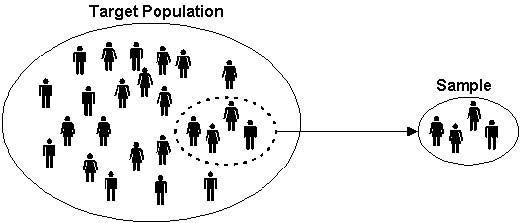
\includegraphics[width=5cm]{figure/target-population.jpg}
\end{center}
\pause \item Compute the sample mean $\xbar$ from the sample
\end{itemize}

\vskip 0.5cm

\pause The \blue{sampling distribution of $\xbar$} 
\begin{itemize}
\pause \item describes how these different instances of $\xbar$ behave
\pause \item has its name because its values are based on \blue{samples}
\end{itemize}

\end{frame}
%------------------------------------------------------------------------------




%-------------------------------------------------------------------------------
\begin{frame}
\frametitle{Sampling Distribution}
Each element in this histogram is one of 1000 instances of $\xbar$ from the previous slide, where each $\xbar$ is computed from a sample of $n=100$ values.  This is the \blue{sampling distribution} of $\xbar$:
\setkeys{Gin}{width=0.65\textwidth}
\begin{center}
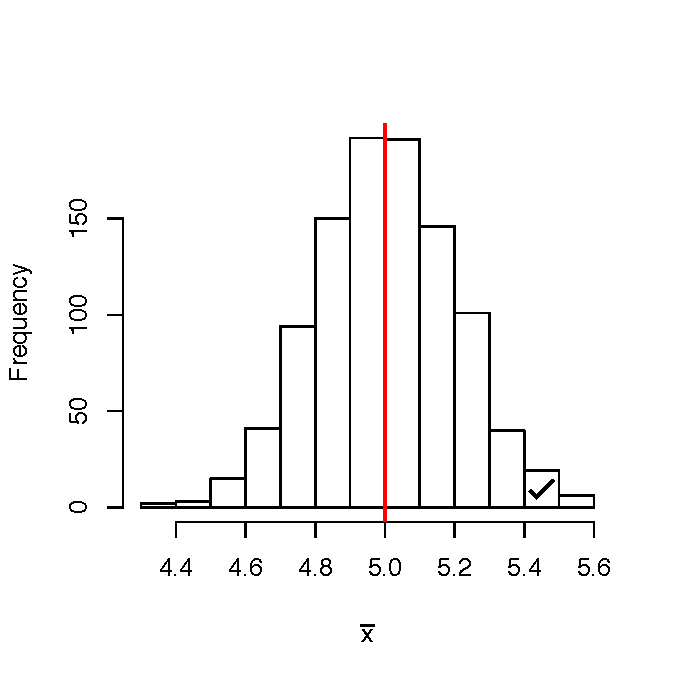
\includegraphics{figure/lec12-001}
\end{center}
\end{frame}
%-------------------------------------------------------------------------------



%-------------------------------------------------------------------------------
\begin{frame}
\frametitle{Behavior of Point Estimates}
Notice in the histogram:
\begin{itemize}
\pause \item the 1000 instances of $\xbar$ are centered around the true population mean $\mu=5$
\pause \item there is a spread of the values about the center.
\end{itemize}

\vspace{0.5cm}

\pause The interval $[4.6, 5.4]$ contains roughly 95\% of the data.  Since
\begin{eqnarray*}
\pause \mbox{the length of the interval } [\mu - 2 SD, \mu + 2SD] &=& 4SD\\
\pause \mbox{the length of the interval } [4.6, 5.4] &=& 4SD\\
\pause 5.4 - 4.6 = 0.8 &=& 4SD\\
\pause SD &=& 0.2
\end{eqnarray*}


\end{frame}
%-------------------------------------------------------------------------------




%------------------------------------------------------------------------------
\begin{frame}[fragile]
\frametitle{Sampling Distributions}

\blue{Definition 2}: the \blue{sampling distribution} is the distribution of point estimates based on samples of fixed size $n$.  

\pause \vspace{0.5cm}

i.e. every instance of a point estimate can be thought of as having been drawn from the sampling distribution.  


\end{frame}
%------------------------------------------------------------------------------





%------------------------------------------------------------------------------
\begin{frame}[fragile]
\frametitle{Standard Errors}

\blue{Definition 3}: The \blue{standard error} is the standard deviation of the sampling distribution of a point estimate.  It describes the uncertainty/variability associated with the point estimate.  

\pause \vspace{0.5cm}

\blue{Very confusing for people}:  the \blue{standard error} is a specific kind of standard deviation.

\pause \vspace{0.5cm}
i.e. it describes the typical \blue{error} in our point estimate $\xbar$.


\end{frame}
%------------------------------------------------------------------------------



%------------------------------------------------------------------------------
\begin{frame}[fragile]
\frametitle{Standard Error of the Sample Mean $\xbar$}

Given $n$ \blue{independent} observations from a population with standard deviation $\sigma$, the \blue{standard error of the sample mean} is
\[
SE = \frac{\sigma}{\sqrt{n}}
\]

\pause A good way to ensure independence of sample observations is to conduct a simple random sample consisting of less than 10\% of the population.  

\end{frame}
%------------------------------------------------------------------------------



%------------------------------------------------------------------------------
\begin{frame}[fragile]
\frametitle{Standard Error of the Sample Mean $\xbar$}


Notice the $\sqrt{n}$ in the denominator: $n$ increases, SE decreases!\\

\pause \vspace{0.5cm}

i.e. as the sample size gets bigger, the variability of our point estimate $\xbar$ decreases.  This is why sample size matters!

\pause \vspace{0.5cm}

Going back to the histogram.  We drew samples of size $n=100$ of data with $\sigma=2$.  We estimated earlier that the standard deviation of the sampling distribution was 0.2.  Using the formula

\[
SE = \frac{\sigma}{\sqrt{n}} = \frac{2}{\sqrt{100}} = \frac{2}{10} = 0.2
\]
\end{frame}
%------------------------------------------------------------------------------



%------------------------------------------------------------------------------
\begin{frame}[fragile]
\frametitle{Standard Error of the Sample Mean $\xbar$}

\[
SE = \frac{\sigma}{\sqrt{n}} = \frac{2}{\sqrt{100}} = \frac{2}{10} = 0.2
\]
\begin{center}
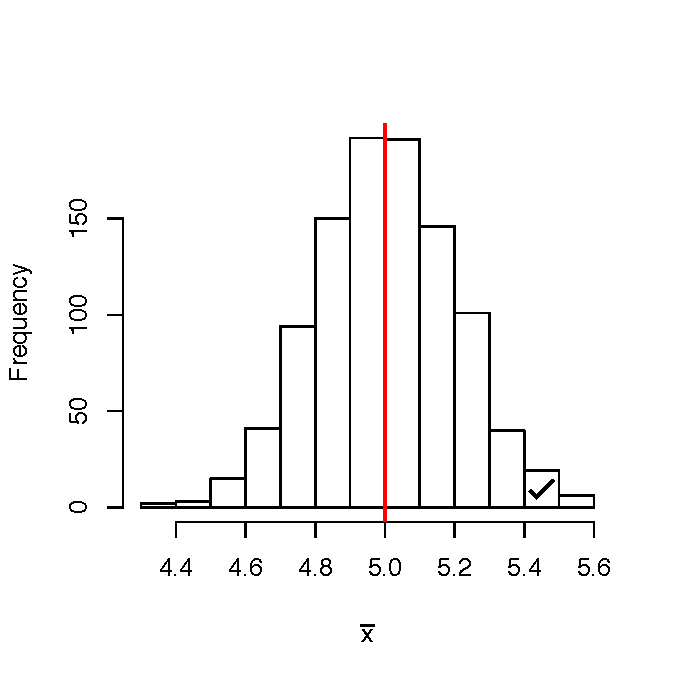
\includegraphics[width=0.55\textwidth]{figure/lec12-001}
\end{center}


\end{frame}
%------------------------------------------------------------------------------




%pdf("./5.2 Variability in Estimates/compare.pdf", height=4.5, width=2*4.5)
%par(mfrow=c(1,2))
%xbar <- rep(0,1000)
%for(i in 1:1000)
%  xbar[i] <- mean(rnorm(n=100,mean=5,sd=2))
%hist(xbar, xlab=expression(bar(x)), main="", xlim=c(4.25, 5.75))
%title("n = 100")
%abline(v=5,col="red",lwd=2)
%
%xbar <- rep(0,1000)
%for(i in 1:1000)
%  xbar[i] <- mean(rnorm(n=1000,mean=5,sd=2))
%hist(xbar, xlab=expression(bar(x)), main="", xlim=c(4.25, 5.75))
%title("n = 1000")
%abline(v=5,col="red",lwd=2)
%dev.off()
%------------------------------------------------------------------------------
\begin{frame}[fragile]
\frametitle{Standard Error of the Sample Mean $\xbar$}
Now compare the sampling distributions based on
\begin{itemize}
\pause \item 1000 instances of $\xbar$ where each $\xbar$ is based on $n=100$.\\
So $SE = \frac{\sigma}{\sqrt{n}} = \frac{2}{\sqrt{100}} = 0.2$
\pause \item 1000 instances of $\xbar$ where each $\xbar$ is based on $n=1000$.\\
So $SE = \frac{\sigma}{\sqrt{n}} = \frac{2}{\sqrt{1000}} = 0.0632$.  \blue{Smaller}!
\end{itemize}

\begin{center}
\pause 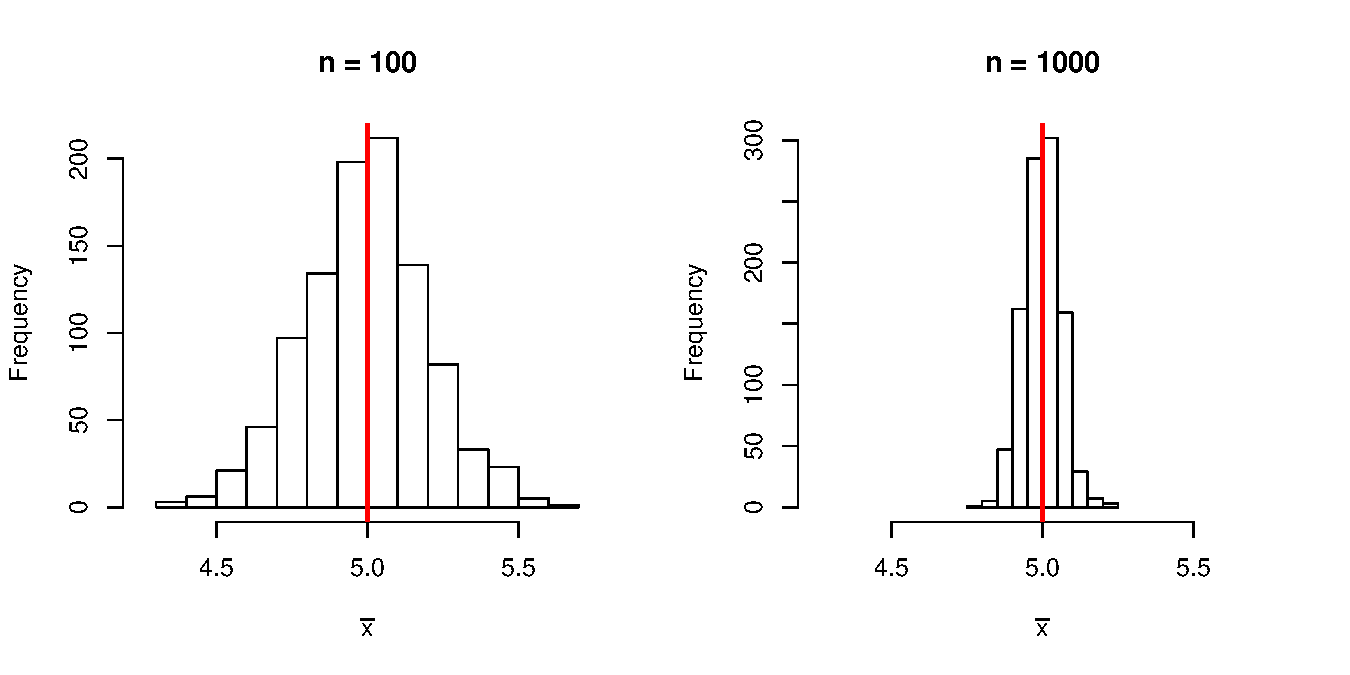
\includegraphics[width=0.9\textwidth]{figure/compare}
\end{center}
\pause The estimates on the right are ``more precise.''

\end{frame}
%------------------------------------------------------------------------------



%------------------------------------------------------------------------------
\begin{frame}[fragile]
\frametitle{Standard Error of the Sample Mean}
In this example we knew $\sigma$.  However, in real life we won't know $\sigma$!

\vspace{0.5cm}

\pause However, when
\begin{itemize}
\pause \item the sample size is at least 30
\pause \item the population distribution is \blue{not} strongly skewed
\end{itemize}
\pause we can use the point estimate of the standard deviation from the sample.  i.e. plug in $s$ in place of $\sigma$:
\[
SE = \frac{s}{\sqrt{n}}
\]

\end{frame}
%------------------------------------------------------------------------------



%------------------------------------------------------------------------------
\begin{frame}[fragile]
\frametitle{Exercise 4.5 on Page 164}

Say in you take a simple random sample of 100 runners and you find:
\begin{itemize}
\item the sample mean $\xbar$ of ages is 35.05
\item the sample standard deviation of the runners ages is $s=8.97$
\end{itemize}

\vspace{0.5cm}

\pause Assuming that the 100 runners consist of less than 10\% of the population (i.e. there are at least 1000 runners in the population), the standard error of the sample mean is 
\[
SE = \frac{s}{\sqrt{100}} = \frac{8.97}{10} = 0.897
\]


\end{frame}
%------------------------------------------------------------------------------


%------------------------------------------------------------------------------
\begin{frame}[fragile]
\frametitle{Sampling Distributions}

We can define the sampling distributions for \blue{any} point estimate, not just $\xbar$:
\begin{itemize}
\item $s$
\item the sample median
\item the sample minimum/maximum
\end{itemize}

\pause We will only focus on sample means, including the sample proportion $\widehat{p}$..

\end{frame}
%------------------------------------------------------------------------------


%------------------------------------------------------------------------------
\begin{frame}[fragile]
\frametitle{Recap}

\begin{itemize}
\pause \item \blue{Point estimates} are based on a sample $x_1, \ldots, x_n$ and are used to estimate population parameters.
\pause \item The \blue{sampling distribution} characterizes the (random) behavior of point estimates.  
\pause \item The standard deviation of a sampling distribution is the \blue{standard error}: it quantifies the uncertainty/variability of point estimates.  
\end{itemize}

\end{frame}
%------------------------------------------------------------------------------


%------------------------------------------------------------------------------
\begin{frame}[fragile]
\frametitle{Next Time}

\begin{itemize}
\item Confidence Intervals
\item When quoting survey results, what does: ``the results of this survey are estimated to be accurate within 3.1 percentage points, 19 times out of 20'' mean?  
\item \blue{Big One}: Central Limit Theorem
\end{itemize}

\end{frame}
%------------------------------------------------------------------------------


\end{document}


